\documentclass[tikz, border=10px]{standalone}
\usepackage{physics}
\usetikzlibrary{automata, positioning, arrows.meta, calc}

\begin{document}
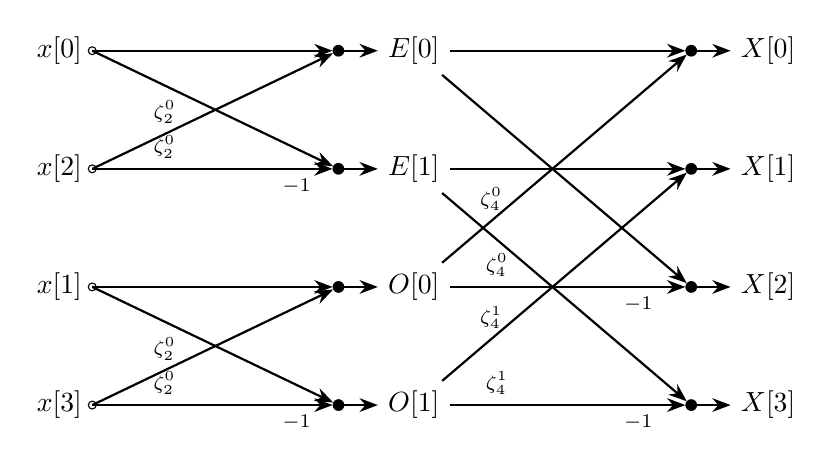
\begin{tikzpicture}[>=Stealth, node distance=1.5cm, thick]

  % --- CONFIGURAÇÕES GERAIS ---
  \def\dy{1.5} 
  
  % Estilo para nós de junção (soma)
  \tikzstyle{junction}=[circle, fill=black, inner sep=1.5pt, outer sep=0pt]

  % --- ENTRADA (Bit-Reversal) ---
  % Pares (Evens)
  \node (x0) at (0, 0) {$x[0]$};
  \node (x2) at (0, -\dy) {$x[2]$};
  % Ímpares (Odds)
  \node (x1) at (0, -2*\dy) {$x[1]$};
  \node (x3) at (0, -3*\dy) {$x[3]$};

  % Círculos nos inputs
  \foreach \n in {x0, x2, x1, x3} {
    \draw [fill=white, thin] (\n.east) circle (0.05);
  }

  % --- SAÍDAS INTERMEDIÁRIAS (E e O) ---
  % Definindo a posição dos nós intermediários
  \node (E0) at (4.5, 0) {$E[0]$};
  \node (E1) at (4.5, -\dy) {$E[1]$};
  \node (O0) at (4.5, -2*\dy) {$O[0]$};
  \node (O1) at (4.5, -3*\dy) {$O[1]$};

  % --- ESTÁGIO 1: BUTTERFLIES (Substituindo os blocos) ---
  
  % -- Butterfly Superior (Entradas x0, x2) --
  % Pontos de junção antes das saídas E
  \node[junction] (jE0) at ($(E0.west) + (-0.5, 0)$) {};
  \node[junction] (jE1) at ($(E1.west) + (-0.5, 0)$) {};

  % Caminhos de x0 (Pares superiores)
  \draw [->] (x0.east) -- (jE0);
  \draw [->] (x0.east) -- (jE1);

  % Caminhos de x2 (Pares inferiores - com Twiddle e -1)
  % Nota: zeta_2^0 é numericamente 1, mas mantido para clareza estrutural.
  \draw [->] (x2.east) -- node[pos=0.3, above, font=\scriptsize] {$\zeta_2^0$} (jE0);
  \draw [->] (x2.east) -- node[pos=0.3, above, font=\scriptsize] {$\zeta_2^0$} node[pos=0.85, below, font=\scriptsize] {$-1$} (jE1);

  % Conectar junções às saídas E
  \draw [->] (jE0) -- (E0);
  \draw [->] (jE1) -- (E1);

  % -- Butterfly Inferior (Entradas x1, x3) --
  % Pontos de junção antes das saídas O
  \node[junction] (jO0) at ($(O0.west) + (-0.5, 0)$) {};
  \node[junction] (jO1) at ($(O1.west) + (-0.5, 0)$) {};

  % Caminhos de x1 (Ímpares superiores)
  \draw [->] (x1.east) -- (jO0);
  \draw [->] (x1.east) -- (jO1);

  % Caminhos de x3 (Ímpares inferiores - com Twiddle e -1)
  \draw [->] (x3.east) -- node[pos=0.3, above, font=\scriptsize] {$\zeta_2^0$} (jO0);
  \draw [->] (x3.east) -- node[pos=0.3, above, font=\scriptsize] {$\zeta_2^0$} node[pos=0.85, below, font=\scriptsize] {$-1$} (jO1);

  % Conectar junções às saídas O
  \draw [->] (jO0) -- (O0);
  \draw [->] (jO1) -- (O1);


  % --- ESTÁGIO 2: COMBINAÇÃO FINAL (Mantido do original) ---
   
  % Nós de Saída Final (X)
  \node (X0) at (9, 0) {$X[0]$};
  \node (X1) at (9, -\dy) {$X[1]$};
  \node (X2) at (9, -2*\dy) {$X[2]$};
  \node (X3) at (9, -3*\dy) {$X[3]$};

  % Pontos de junção para o estágio final
  \node[junction] (jX0) at ($(X0.west) + (-0.5, 0)$) {};
  \node[junction] (jX1) at ($(X1.west) + (-0.5, 0)$) {};
  \node[junction] (jX2) at ($(X2.west) + (-0.5, 0)$) {};
  \node[junction] (jX3) at ($(X3.west) + (-0.5, 0)$) {};

  % Conectar junções às saídas finais
  \foreach \n in {0,1,2,3} { \draw[->] (jX\n) -- (X\n); }

  % Linhas retas (Pares vêm de E)
  \draw [->] (E0) -- (jX0); % E[0] -> X[0]
  \draw [->] (E1) -- (jX1); % E[1] -> X[1]
  \draw [->] (E0) -- (jX2); % E[0] -> X[2]
  \draw [->] (E1) -- (jX3); % E[1] -> X[3]

  % Linhas cruzadas (Ímpares vêm de O com Twiddle Factors)
  % O[0] caminhos
  \draw [->] (O0) -- node[above, pos=0.2, font=\scriptsize] {$\zeta_4^0$} (jX0); 
  \draw [->] (O0) -- node[above, pos=0.2, font=\scriptsize] {$\zeta_4^0$} node[below, pos=0.8, font=\scriptsize] {$-1$} (jX2);

  % O[1] caminhos
  \draw [->] (O1) -- node[above, pos=0.2, font=\scriptsize] {$\zeta_4^1$} (jX1); 
  \draw [->] (O1) -- node[above, pos=0.2, font=\scriptsize] {$\zeta_4^1$} node[below, pos=0.8, font=\scriptsize] {$-1$} (jX3);

\end{tikzpicture}
\end{document}
